\documentclass[11pt]{article}
\usepackage[margin=0.85in]{geometry}
\usepackage{amsmath,amssymb,graphicx,xurl,hyperref}
\setlength{\parindent}{0pt}\setlength{\parskip}{7pt}
\begin{document}
{\LARGE Actual prescribed quotient-buffer capacity}\par
November9,2026. Source \texttt{8e62d4dfc}. Unsigned producer evidence
[pcc:unverified].

\textbf{Exact accounting.} Let $B$ count all prescribed coefficient slot
widths, one quotient vector per actual node. For $0<u\leq a$ and
$h=\lceil3M/u\rceil$, Lean identifies the actual-node sum with
\[
 B=\sum_{i=0}^{u-1}2^{a-i}h(u-i)
       \bigl[p+8h2^{a-i}+8M(a+1)\bigr].
\]
Actual valuation cardinalities supply each level count. The zero node and
inactive levels have zero order. Keeping only the odd-node level gives
\[
 B\geq 8h^2u4^a,\qquad uB\geq72M^2 4^a.
\]
The second inequality uses the actual source ceiling $hu\geq3M$.

\textbf{Meaning of the charge.} Simultaneous fixed-width packed storage of
all those prescribed slots charges at least $B$ bits. This is a capacity
accounting convention, including slots whose value is zero. It is not an
information-theoretic lower bound against streaming, sparse or compressed
representations, shared storage, alternate precision schemes or other
algorithms. No RSS, allocation or timing measurement has been taken.

\textbf{Parameter implication.} For input length $n$, a linear grid exponent
$a$ makes this simultaneous capacity exponential through $4^a$, since
$u\leq a$. A sub-exponential version of this explicit strategy needs a
sublinear grid exponent or a representation avoiding simultaneous capacity.
This condition is necessary for this strategy and gives no sufficient
recursive runtime theorem. The manuscript uses $\lambda=\lceil\log_2 s\rceil$
and $a\leq4\epsilon\lambda$, hence $L\leq s^{1/1000}$. Its intended
$4^a=L^2$ factor is polynomial in $s$; this bound does not reject that schedule.

\textbf{Auxiliary algebra.} The formal weighted sum
$W_r(u)=\sum_{j=0}^{u-1}(j+1)r^j$ satisfies
\[
 (r-1)^2W_r(u)=[u(r-1)-1]r^u+1.
\]
Specializations $r=2,4$ are available; connecting a fully closed form for $B$
is a separate next step.
\newpage
{\Large Dependency map and evidence}\par
\begin{center}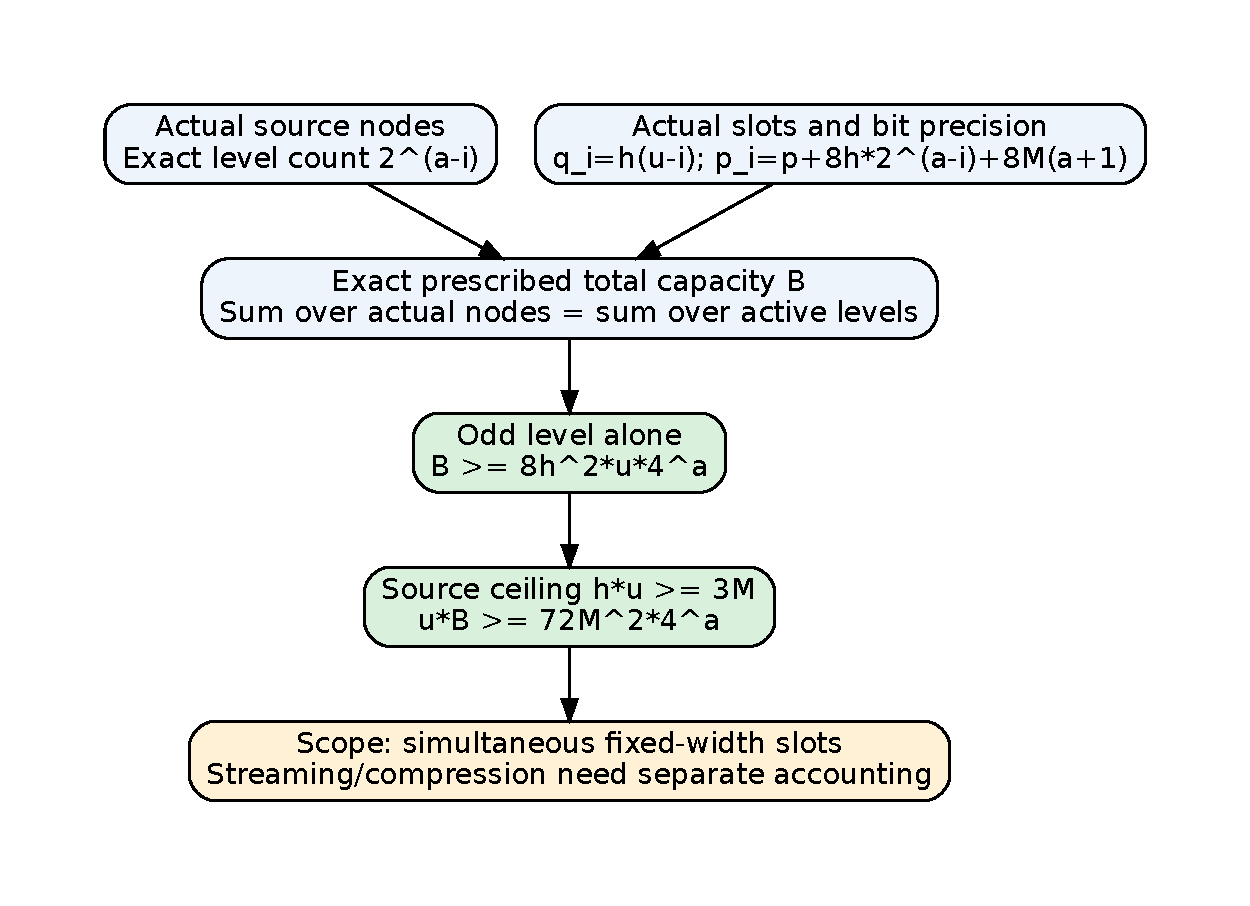
\includegraphics[width=0.96\linewidth,height=0.58\textheight,keepaspectratio]{budget.pdf}\end{center}

\textbf{Source bindings.} \texttt{BufferBudget.actualBufferBitsEq},
\texttt{actualBufferBitsLower}, \texttt{actualBufferBitsPortLower} and
\texttt{weightedIdentity}. Their canonical PCC pins and final audit/replay
receipts are linked by the companion Markdown report. Failed build002 is
retained; successful builds003/004 contain no unsolved declarations.

\textbf{Sources and continuation.} Actual node counts, source orders and
child precision from the preceding formal recovery component; pinned
manuscript D.9/D.10 as cited there. KB unavailable (wrapper has no executable).
Native census protocol is prospectively frozen; S3 admission failed for missing
transport and no data was collected. Continue parameter/cost derivation while
that experiment-only dependency is resolved. Streaming needs separate retained
state and recomputation bounds.
\end{document}
